\section{Webserver}

Damit die vom Arduino ermittelten Standortdaten des Fahrzeugs an die Apps weitergeleitet werden können, benötigt es eine Zwischeninstanz. Diese soll die empfangenen Daten aufbereiten und sie anschließend so bereitstellen, dass sie einfach von den Apps abgefragt werden können.
In einem zweiten Entwicklungsschritt soll dann der Sicherheitsaspekt der Daten berücksichtigt werden. Hierfür sollen Verschlüsselungsalgorithmen implementiert werden, sodass die Daten nur von den Apps entschlüsselt und ausgewertet werden können.

\subsection{Einrichtung des Webservers auf einem Raspberry Pi}
Der HTTP-Webserver soll auf einem Raspberry Pi mit Hilfe des „lighttpd“-Webservers erstellt werden. Die Installation und Einrichtung desselbigen gestaltete sich relativ einfach. Zunächst musste das entsprechende „lighttpd“-Paket auf dem Raspberry Pi installiert werden. Im nächsten Schritt mussten noch ein paar Berechtigungen erteilt werden. Nach einem Neustart von lighttpd war die Einrichtung soweit fertig und der Webserver war aktiv. Alle Dateien und Skripte, die der Webserver bereitstellt und bearbeitet liegen im Verzeichnis „/var/www/html“.
\\
Damit der Server später auch von außerhalb erreichbar ist, waren noch einige Arbeitsschritte zu erledigen. Zuerst musste der Raspberry Pi eine statische IPv4-Adresse erhalten, wir setzten diese auf 192.168.178.215. Die .215 wurde deshalb ausgewählt, weil der Bereich der automatischen Adresszuweisung von den meisten DHCP-Servern nur von .0 bis .200 geht und somit eine doppelte Vergabe sehr unwahrscheinlich ist.
\\
Bei DYNDNS handelt es sich um einen Service, der es ermöglicht, Domains mit dynamisch wechselnden IP-Adressen im Internet zu verwalten. Dieser Service ist notwendig, da der heimische Router vom Provider in regelmäßigen Abständen eine neue, externe IP-Adresse zugeordnet bekommt und somit der Raspberry Pi bzw. der darauf aktive Webserver nach einem "IP-Wechsel" nicht mehr über das Internet erreichbar wäre. Bei Nutzung eines DYNDNS Anbieters, bleibt der Raspberry Pi bzw. der Webserver weiterhin unter seinem vergebenen Hostnamen erreichbar. Damit ein solcher Service genutzt werden kann, ist es notwendig, sich bei einem DYNDNS-Anbieter einen Account anzulegen. Für diese Arbeit wurde sich aufgrund einer persönlichen Empfehlung für Securepoint DYNDNS entschieden. Auf deren Webseite konnte nach der Erstellung eines Benutzerkontos ein IPv4-Host hinzugefügt werden. Dafür wurde neben der IP-Adresse des Raspberry Pi der Hostname eingetragen, welcher dann automatisch eine Domainerweiterung des DYNDNS Anbieters erhalten hat.
\\
Im letzten Schritt musste nun der heimische Router so konfiguriert werden, dass ein Zugriff auf den Webserver von außerhalb des Heimnetzwerks erlaubt ist. In unserem Fall handelt es sich beim Router um eine FRITZ!Box, bei welcher diese Einstellungen einfach vorgenommen werden konnten.  Dafür musste zunächst eine neue Freigabe für das Gerät „Raspberry Pi“ hinzugefügt werden. Anschließend wird als Anwendung „HTTP-Server“ und damit Port 80 ausgewählt. Zusätzlich musste dann noch das DYNDNS in der FRITZ!Box konfiguriert werden. Dafür wird eine Update-URL des DYNDNS-Anbieters sowie der Domainname und die Benutzerinformationen benötigt. Damit waren alle notwendigen Einstellungen vorgenommen und er Webserver ist nun von überall erreichbar.
\\
Zusätzlich haben wir die Software „VNC Server“ auf dem Raspberry Pi installiert. Mit Hilfe dieser Software und dem entsprechenden Client „VNC Viewer“ auf einem PC oder Laptop kann eine Remotedesktopverbindung zum Raspberry Pi hergestellt werden. Dies ist besonders auch in Zeiten von Lockdowns und Online-Vorlesungen sowie digitalen Gruppenmeetings eine wichtige Funktion, da so von überall an dem Raspberry Pi gearbeitet werden kann.

\subsection{Probleme mit dem Raspberry Pi}
Während der ersten Wochen der Projektarbeit mussten wir leider alle paar Tage feststellen, dass keine Verbindung per VNC zum Raspberry Pi hergestellt werden konnte. Wir vermuteten zunächst keinen dramatischen Fehler, denn nach einem Neustart funktionierte wieder alles. Dieser Fehler trat allerdings doch mit einer gewissen Regelmäßigkeit auf und nachdem ein erstes PHP-Skript auf unserem Webserver lief, konnten wir feststellen, dass dieses auch regelmäßig nicht erreichbar war. Der Fehler lag also eindeutig nicht nur an der VNC-Software, sondern es scheint generelle Verbindungsprobleme des Raspberry Pi zu geben.
Deshalb versuchten wir doch genauer herauszufinden, wo der Ursprung des Verbindungsverlustes ist. Nach einigem Recherchieren und dem Sichten diverser Log-Files auf dem Raspberry Pi konnten wir die Fehlermeldung „brcmf\_cfg80211\_scan: scan error (-110)“ für die Verbindungsabbrüche ausfindig machen. Bei diesem Fehler handelt es sich um ein Verbindungsproblem des WiFis des Raspberry Pi’s. Dieser Fehler ist nicht unbekannt und mögliche Lösungen werden in diversen Internetforen diskutiert. Allerdings scheint keine der vorgeschlagenen Workarounds generell zu funktionieren, außer ein wie auch von uns praktiziertes, regelmäßiges Neustarten. Bevor wir diese alle ausprobieren und im ungünstigsten Fall eine Menge Zeit ohne Ergebnis verschwenden würden, entschlossen wir uns einfach dazu, den Raspberry Pi per LAN-Kabel direkt mit der Fritzbox zu verbinden. Nachdem dann auch nach über zwei Wochen keine Verbindungsabbrüche registriert wurden, konnten wir dieses Problem als gelöst ansehen und uns wieder anderen Aufgaben des Projekts widmen.
\\
Im Verlauf der weiteren Programmierung der PHP-Skripte stellte sich heraus, dass die PHP-Version 7.3 auf dem Raspberry Pi veraltet war und einige nützliche Funktionen nicht unterstützt. Deshalb wurde die Version 7.3 deinstalliert und anschließend mit PHP 8.0 eine der aktuellen Versionen installiert. Allerdings lief entweder die Deinstallation der alten oder die Installation der neuen Version nicht fehlerfrei. Nach einigem Suchen in verschiedenen Log-Files stellte sich heraus, dass fälschlicherweise die Socket-Datei „php7.3-fpm.sock“ der Version 7.3 vom lighttpd-Server versucht wurde zu öffnen. Diese existierte aber natürlich nach der Deinstallation nicht mehr. Mit PHP 8.0 wurde eine entsprechende, neue Datei „php8.0-fpm.sock“ im gleichen Dateipfad „/var/run/php“ bereits erzeugt. In der Konfigurations-Datei „15-fastcgi-php.conf“ im Verzeichnis „/etc/lighttpd/conf-enabled“ ist der Pfad der vom lighttpd-Server zu nutzenden Socket-Datei hinterlegt. Allerdings ist es nicht möglich, diese Datei einfach mit Hilfe eines Texteditors auf dem Raspberry Pi zu verändern. Dafür benötigt es höhere Benutzerrechte. Die Datei lässt sich auch über die Kommandozeile öffnen und bearbeiten. Dabei ist es wichtig den Zusatz „sudo“ vor jeden Befehl zu schreiben, da somit für den folgenden Befehl die notwendigen höheren Rechte temporär gewährt werden. So war es möglich, in der Datei „15-fastcgi-php.conf“ den Pfad der Socket-Datei auf die aktuelle Datei von PHP-Version 8.0 zu ändern. Im Anschluss musste der lighttpd-Server noch einmal neu gestartet werden, sodass alle Änderungen übernommen werden konnten.

\subsection{Grundsätzliche Überlegungen}
Bevor es ans konkrete Programmieren verschiedener HTML- oder PHP-Skripte geht, wollte wir uns zunächst überlegen, was denn grundsätzlich auf dem Server passieren soll. Auf jeden Fall benötigen wir ein Skript, das Daten nutzen und weiterverarbeiten kann, die an seine URL (Uniform Resource Locator) übermittelt wurden. Darüber hinaus ist es sicherlich sinnvoll und möglicherweise sogar notwendig, das Bereitstellen von Daten für die Apps in einem separaten Skript zu realisieren. Zusätzliche Skripte für zum Beispiel eine Verschlüsselung der Daten sind gegebenenfalls zu einem späteren Zeitpunkt noch interessant.
Auch wenn der GPS-Sensor am Arduino neben den Längen- und Breitengraden noch viele andere Informationen erfasst, reicht es für unser primäres Projektziel aus, nur die Koordinaten an den Webserver zu senden. Um die Koordinaten-Paare bei der Weiterverarbeitung in den Apps unterscheiden zu können, soll der Webserver die Daten noch mit dem aktuellen Zeitstempel verknüpfen.
\\
Sowohl die Daten, die der Arduino an den Webserver übermittelt als auch die Daten, die der Webserver für die Apps wieder bereitstellt, sollen im JSON-Format (JSON = JavaScript Object Notation) übertragen werden. Dieses Format ist einerseits leicht lesbar und andererseits ist es unabhängig von Programmiersprachen und somit universell nutzbar.
\\
Über mögliche Sicherheitsaspekte unserer Datenübertragung dachten wir anfangs nicht wirklich nach, da eine an sich funktionierende Kommunikation zwischen den verschiedenen Teilnehmern erstmal im Vordergrund stand. Lediglich die Überlegung, wie man verhindern kann, dass nicht jeder beliebige Internetnutzer irgendwelche Daten an unseren Webserver schickt, beschäftigte uns am Anfang des Projekts. Es lässt sich natürlich nicht verhindern, dass andere Geräte versehentlich oder auch absichtlich irgendwelche Daten an unseren Webserver bzw. an ein dort laufendes PHP-Skript senden. Aber wir können dieses Skript so programmieren, dass nur bestimmte empfangene Daten auch weiterverarbeitet werden. Um dies zu realisieren, muss jedes Gerät eine von uns manuell vergebenen Geräte-Identifikationscode (Geräte-ID) zusammen mit den Nutzdaten verschicken. Diese Geräte-IDs sind 20-stellige, alphanumerische Werte, die wir einmal zufällig generiert haben und die in der txt-Datei „allowed\_devices.txt“ lokal auf dem Raspberry Pi gespeichert sind. So kann später darauf zugegriffen werden und ein Abgleich erfolgen, ob die mitgesendete Geräte-ID bei uns bekannt ist. Wenn dies nicht der Fall ist, sollen diese Daten nicht weiterbearbeitet werden.
\\
Es ist klar, dass auch diese Sicherheitsvorkehrung nicht besonders stark ist, solange die Geräte-IDs unverschlüsselt und quasi frei zugänglich auf dem Server gespeichert sind. Aber es ist ein erstes Mittel, um zumindest einfache Störversuche zu unterbinden und auch uns selbst vor möglichen Übertragungsfehlern zu schützen.
\\
Es ist sehr wahrscheinlich, dass nicht alle Projektteile mit der gleichen Geschwindigkeit bearbeitet werden und somit einzelne Teile unterschiedlich schnell in einem testfähigen Stadium sind. In diesem Fall betrifft das die GSM-Sendeeinheit des Arduinos und die einzelnen Skripte des Webservers. Damit grundsätzliche Funktionalitäten der Skripte möglichst schon während der Entwicklung getestet werden können, ohne dass erst auf den Projektteil des Arduinos gewartet werden muss, wollten wir eine einfache Anwendung für einen Windows-PC entwickeln. Die Entscheidung fiel hier relativ schnell auf die Programmiersprache Python, da wir diese auch schon zuvor in einigen Studienprojekten benutzt hatten und sie für den hier gedachten Einsatzzweck eine einfache und schnelle Umsetzung verspricht.

\subsection{Testprogramme}
Im Verlauf der Programmierung der PHP-Skripte auf dem Webserver wurden insgesamt drei Python-Skripte geschrieben, um die Funktionen auf dem Webserver zu testen.
\\
Das erste Python-Skript heißt „Senden.py“. Mit ihm soll getestet werden, ob gesendete Daten beim Webserver ankommen und auch weiterverarbeitet werden können. Dafür werden neben einer gültigen Geräte-ID auch je eine Variable für den Breitengrad (Latitude) und den Längengrad (Longitude) mit frei gewählten Startwerten deklariert. Ebenso wird die URL des empfangenden Skripts auf dem Webserver („http://retrorbit.spdns.de/get\_Data.php“) als Variable gespeichert. Der restliche Code ist eine endlose while-Schleife, in der die aktuellen Daten ins JSON-Format gebracht und dann mittels HTTP-POST an die gespeicherte URL gesendet werden. Danach folgt noch eine kurze Wartezeit von 5 Sekunden sowie eine Inkrementierung der Latitude und eine Dekrementierung der Longitude jeweils um den Wert 1.
\\
Im zweiten Python-Programm mit dem Namen „Abfragen.py“ werden innerhalb einer endlosen while-Schleife die aktuellen Werte vom Webserver bzw. von der Webseite „http://retrorbit.spdns.de/provide\_Data.php“ per HTTP-GET abgefragt und die Daten im JSON-Format ausgegeben.
\\
Das dritte Python-Skript heißt „Störer.py“ und gleicht dem „Senden.py“-Skript. Mit diesem sollten zeitgleich entweder beliebige oder auch vom Format her gleiche Werte an das „get\_Data.php“-Skript gesendet werden. So wollten wir überprüfen, ob die Sicherheitseinrichtung mit den Geräte-IDs tatsächlich funktioniert.

\subsection{Erstellen der PHP-Skripte zum Empfangen und Bereitstellen von Daten}
\textbf{Erläuerungen zum Code }Bei allen drei übermittelten Parametern, also Geräte-ID, Latitude und Longitude, wird immer eine Prüfung durchgeführt, bevor deren Werte tatsächlich in Variablen des PHP-Skripts geschrieben werden. Die Struktur dieser Prüfung ist bei allen drei Parametern identisch, bis auf den entsprechenden Bezeichner und den Variablennamen.
Die Variable übernimmt nur dann den Wert der \$POST Daten, wenn diese einerseits von „null“ verschieden sind und andererseits nicht leer sind. Dies wird realisiert, indem in einer if-Abfrage das Ergebnis der „isset“-Funktion mit der Bedingung, dass der \$POST Wert ungleich leer ist, über ein logisches UND verknüpft sind. Die „isset“-Funktion prüft dabei, ob die Variable existiert und sich von „null“ unterscheidet. Wenn diese Bedingungen allerdings nicht erfüllt sind, wird im else-Zweig mittels goto-Anweisung zum Ende des Skriptes gesprungen und eine Fehlermeldung ausgegeben. Die aktuell empfangenen Daten werden dann nicht weiterverarbeitet, sodass immer noch der vorherige Standort von der Seite „http://retrorbit.spdns.de/provide\_Data.php“ abgefragt werden kann.
\\
Mit der Funktion str\_contains kann überprüft werden, ob ein String in einem anderen String enthalten ist. In unserem Fall wird so gecheckt, ob die Geräte-ID (\$device\_id) im String \$all\_devices enthalten ist, welcher alle Geräte-IDs aus der Datei „allowed\_devices.txt“ beinhaltet.
\\
Die aus den \$POST Variablen übernommenen Werte für Latitude und Longitude werden dann zusammen mit den aktuellen Datumsinformationen in ein Array mit der Bezeichnung \$koor kopiert. Anschließend wird dieses Array noch in JSON codiert und als \$json\_koor gespeichert. Wichtig ist an dieser Stelle der zweite Parameter des json\_encode Befehls. Wenn hier nichts angegeben wird, werden alle enthaltenen Werte als String interpretiert. Für das Datum und die Uhrzeit ist das sinnvoll, für die Koordinaten hingegen eher nicht. Damit deren Werte auch als Zahlenwerte interpretiert werden, ist der Parameter „JSON\_NUMERIC\_CHECK“ zu setzen, welcher automatisch Zahlenformate erkennt und ins JSON Format übernimmt. Im letzten Schritt des „get\_Data.php“ Skripts wird der aktuelle Inhalt der Datei „Koordinaten.txt“ mit den Daten der JSON-codierten Variable \$json\_koor überschrieben.
\\
Die Trennung für Datenempfang und Datenbereitstellung hat folgenden wichtigen, technischen Hintergrund. In dem Moment, in dem ein http-Request an das „get\_Data.php“ Skript gestellt wird – egal ob Daten mittels POST dorthin übermittelt werden oder nur die bereitgestellten Daten mittels GET abgefragt werden sollen – wird es einmal ausgeführt. Da bei einer reinen GET-Abfrage aber natürlich keine Daten mitgeschickt werden, wird der entsprechende PHP-Code zur Datenverarbeitung übersprungen und die Koordinaten mit „null“ gefüllt. Genau dies wird danach auch ausgegeben und von dem http-GET-Request ausgelesen. Somit ist es nicht möglich innerhalb eines PHP-Skripts Daten zu empfangen und bereitzustellen.
\\
In der nachfolgenden Abbildung ist der grundsätzliche Programmablauf der beiden PHP-Skripte auf dem Webserver dargestellt, die die Datenverarbeitung sowie die Datenbereitstellung realisieren.
\begin{figure} [H]
	\begin{center}
		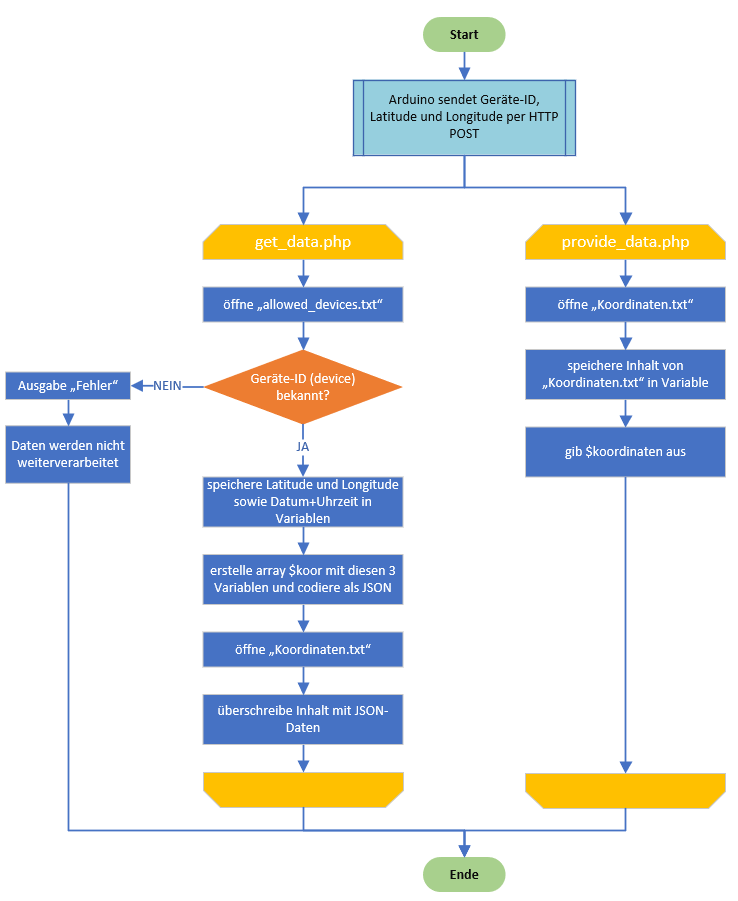
\includegraphics[width=1\textwidth]{Bilder/Webserver_PAP.png}
		\caption{Programmablaufplan Webserver}
		\label{server-pap}
	\end{center}
\end{figure}
\textbf{Probleme beim Senden vom Arduino }Nachdem das Skript „get\_Data.php“ in einem funktionsfähigen Zustand war und auch das Testen mit dem Python-Programm „Senden.py“ keine Fehler ergab, konnte zum nächsten Entwicklungsschritt übergegangen werden. Dieser besteht darin, die Kommunikation vom Arduino über das GSM-Modul zum Webserver herzustellen, sodass dort die gesendeten Daten auch weiterverarbeitet werden können.
Im Prinzip müssen im Programm auf dem Arduino nur die Koordinaten ins JSON Format gebracht werden und per http-POST an die URL „http://retrorbit.spdns.de/get\_Data.php“ gesendet werden. Es erforderte einige Versuche, bis das überhaupt funktionierte, allerdings konnten die Daten auf dem Webserver nicht richtig verarbeitet werden. Dies äußerte sich darin, dass in der Datei „Koordinaten.txt“ für Latitude und Longitude der Wert „null“ eingetragen war. Das Auslesen der Daten mittels POST auf der Seite des Webservers hat also nicht funktioniert. Die Ursache hierfür lag bei der Datenformatierung des Arduinos bzw. dem AT-Befehl zum Senden der Daten via GSM. Dabei werden die Daten immer als String versendet unabhängig von der ursprünglichen Form, welche dann als String angesehen wird. Deshalb funktionierten im PHP-Skript die \$\_POST Befehle für die einzelnen Parameter nicht mehr.
\\
Mit diesem Wissen wurde das „get\_Data.php“ Skript nochmals angepasst und als „get\_Data2.php“ abgespeichert. Dieses ist im Prinzip genauso aufgebaut wie die ursprüngliche Version, jedoch wurden die einzelnen \$\_POST Befehle gegen einen normale Arraybezeichner (\$POST\_data) ausgetauscht. Dafür wird nach den Deklarationen der Dateinamen in Zeile 6 mit nur einem  \$\_POST der vom Arduino gesendete String ausgelesen und in der Variable \$Arduino\_Daten gespeichert. Es folgt eine JSON-Decodierung, sodass nun die einzelnen Parameter (Geräte-ID und die beiden Koordinaten) im Array \$POST\_data gespeichert und referenzierbar sind. Der Zugriff auf die einzelnen Werte geschieht jetzt also nicht mehr über die \$\_POST Befehle, sondern per Referenzierung auf das Array.

\subsection{Verschlüsselung der Daten}
\textbf{Hintergrund }Im aktuellen Zustand des Webservers und unserer Kommunikation allgemein werden die Koordinaten unverschlüsselt und damit für jedes Gerät bzw. jeden Nutzer klar lesbar auf der Seite
 \begin{center}
 	\textit{http://retrorbit.spdns.de/provide\_Data.php }
 \end{center}
 dargestellt. Sowohl aus datenschutztechnischer Sicht als auch im Interesse des späteren Kunden ist dies natürlich nicht. Deshalb ist es nötig, die bereitgestellten Daten zu verschlüsseln. Der wichtigste Punkt an dieser Stelle ist, dass die verwendeten Chiffrier- und Dechiffrieralgorithmen bzw. Bibliotheken sowohl von PHP als auch von den beiden Programmiersprachen der Apps unterstützt werden.
\\
\textbf{Symmetrische und asymmetrische Verschlüsselungsverfahren }Die Verschlüsselung unserer Nutzdaten, also Latitude, Longitude sowie die dazugehörigen Datumsinformationen, soll mittels eines symmetrischen Verschlüsselungsverfahren realisiert werden. Symmetrische Verschlüsselungs-verfahren sind einerseits sehr performant, selbst bei großen Datenmengen, und andererseits sind sie nur unter unverhältnismäßig großem Aufwand zu entziffern. Ein weit verbreiteter, frei verfügbarer Standard stellt dabei der „Advanced Encryption Standard“, kurz AES, den auch wir bei unserem Projekt nutzen wollen. Bei symmetrischen Verschlüsselungsverfahren wird für das Ver- und Entschlüsseln ein und derselbe Schlüssel benutzt. Beim AES kann dieser Schlüssel wahlweise 128, 192 oder 256 Bit lang sein, wobei gilt: Je länger der Schlüssel ist, desto höher ist auch die Sicherheit der verschlüsselten Daten. Bei der symmetrischen Verschlüsselung besteht aber ein wesentlicher Nachteil, denn der Schlüssel muss beiden Teilnehmern der Kommunikation bekannt sein. Wenn die Chiffrierung also auf Gerät A durchgeführt wird, muss neben den nun verschlüsselten Daten auch der AES-Schlüssel zu Gerät B übertragen werden. Je nach individuellen Gegebenheiten lässt sich dies ggf. auf einem zweiten Kommunikationsweg manuell durch den Menschen realisieren. In der Praxis ist das aber meist nicht möglich. Deshalb wird hier zusätzlich noch ein asymmetrisches Verschlüsselungsverfahren angewandt, mit welchem der AES-Schlüssel chiffriert wird. Diese Kombination beider Verschlüsselungsverfahren wird auch als Hybride Verschlüsselung bezeichnet.
\\
Bei asymmetrischen Verschlüsselungsverfahren hat jeder Kommunikationspartner ein eigenes Schlüsselpaar bestehend aus einem öffentlichen und einem geheimen Schlüssel. Der öffentliche Schlüssel wird immer für die Verschlüsselung von Daten beim jeweilig anderen Teilnehmer genutzt und der geheime Schlüssel für die Entschlüsselung der empfangenen Daten auf dem eigenen Gerät. Der Vorteil ist hier, dass der öffentliche Schlüssel bei der Übermittlung an den Kommunikationspartner nicht extra geschützt werden muss. Eines der bekanntesten asymmetrischen Verschlüsselungsverfahren ist das nach seinen Entwicklern benannte RSA-Verfahren. Da dieses aber schon veraltet ist, werden wir mit der Elliptic Curve Cryptography ein zeitgemäßeres Verfahren nutzen.
\\
\textbf{Implementierung der Verschlüsselung auf dem Webserver }Der komplette Verschlüsselungsprozess ist in „encryption.php“ realisiert, also sowohl die Verschlüsselung der Nutzdaten als auch die Chiffrierung des AES-Schlüssels. Für die Übermittlung des öffentlichen Schlüssels wird zusätzlich das Skript „key\_from\_app.php“ erstellt. Allerdings ist die Implementierung noch nicht im Zusammenspiel mit einer der Apps getestet worden, da es hier Verzögerungen im Projekt gab, sodass das ganze Verschlüsselungsthema erst in naher Zukunft tatsächlich funktionsfähig sein wird. Für die symmetrische Verschlüsselung nutzen wir in PHP die Funktionen der „OpenSSL“ Bibliothek und für die asymmetrische Verschlüsselung kommen die Funktionen der „Sodium“ Bibliothek zum Einsatz, welche auch für die von uns verwendeten Programmiersprachen der Apps zur Verfügung stehen.
\\
Als erstes werden die zu verschlüsselnden Nutzdaten (Koordinaten und Datum mit Uhrzeit) aus der Datei „Koordinaten.txt“ geladen. Anschließend wird das Verschlüsselungsverfahren auf AES-192-CTR festgelegt und ein entsprechend langer AES-Schlüssel generiert. CTR steht dabei für Counter Mode, welcher zusätzlich einen Initialisierungsvektor erfordert, welcher die gleiche Länge wie der AES-Schlüssel haben muss. Nachdem dieser Initialisierungsvektor generiert wurde, folgt die eigentliche Verschlüsselung unserer Nutzdaten mit der Funktion „openssl\_encrypt“. Weiter geht es mit der Generierung des Schlüsselpaares des Webservers für die asymmetrische Verschlüsselung mit der Funktion „sodium\_crypto\_box\_keypair()“.
\\
Nun fehlt noch der öffentliche Schlüssel aus der App. Dieser wird aus der Datei „app\_key.txt“ geladen. Diese Datei wurde im Skript „key\_from\_app.php“ generiert und lokal auf dem Server gespeichert. Dieses Skript ist im Prinzip genau so aufgebaut wie das „get\_Data.php“ Skript, nur dass es entsprechend nur auf die beiden Parameter „Geräte-ID“ und „keypair2\_public“ abgestimmt ist. So findet auch hier zuerst eine Überprüfung statt, ob die gesendeten Daten von einem bekannten, erlaubten Gerät stammen.
\\
Nachdem dann also alle notwendigen Schlüssel auf dem Webserver vorhanden sind, kann der AES-Schlüssel mit der Funktion „sodium\_crypto\_box()“, welche noch eine zusätzliche Zufallszahl (nonce) benötigt, verschlüsselt werden. Diese Zufallszahl wurde zuvor erzeugt und muss auch an den Empfänger für die Entschlüsselung übermittelt werden. Im nächsten Schritt werden wieder alle zu sendenden Variablen in ein Array (\$datenpaket) kopiert, siehe untenstehende Abbildung. Dabei ist es wichtig, dass alle Variablen bis auf die verschlüsselten Nutzdaten noch einmal mit base64 codiert werden, da sonst bei der JSON-Codierung des Arrays im nächsten Schritt nicht alle Zeichen der einzelnen Strings korrekt verarbeitet werden können. Bevor diese Strings dann allerdings in den Apps genutzt werden können, muss dort wieder eine base64 Decodierung erfolgen, um wieder das BYTES Format zu erhalten.
\\
Im letzten Schritt werden nun die JSON codierte Variable \$json\_data in der Datei „Datenpaket.txt“ lokal abgespeichert. Diese Datei kann dann genau wie zuvor die Datei „Koordinaten.txt“ von dem Skript „provide\_Data.php“ geöffnet und deren Inhalt ausgegeben werden. So können die Entschlüsselungsparameter zusammen mit den verschlüsselten Daten von den Apps abgefragt werden.
\begin{figure} [H]
	\begin{center}
		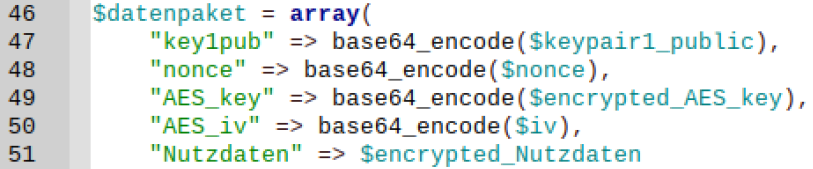
\includegraphics[width=1\textwidth]{Bilder/Webserver_verschluesslung.png}
		\caption{Datenpaket Webserver}
		\label{server-dp}
	\end{center}
\end{figure}
Der gesamte Ablauf der Skripte auf dem Webserver ist in der nachfolgenden Übersicht zur besseren Nachvollziehbarkeit noch einmal schematisch dargestellt.
\begin{figure} [H]
	\begin{center}
		\includegraphics[width=1\textwidth]{Bilder/Webserver_pap2.jpg}
		\caption{Skriptablauf Webserver}
		\label{server-script}
	\end{center}
\end{figure}

